\section{MIPS Assembler Compiler}
\label{sec:MIPS}
\subsection{Introduction}
Before embarking upon this project, very little was known about the MIPS architecture and code generation, in general. These were the main areas that were researched. The code generator that was produced takes in a list of Three Address Code instructions (as described fully in section \ref{sec:tacintro}) and outputs MIPS code that is designed to be run in the SPIM emulator\footnote{\url{http://pages.cs.wisc.edu/~larus/spim.html}}. MIPS code can be generated for most input programs, but for a few exceptions that will be mentioned at the end of this section. The main body of the code generator is another recursive procedure which walks the list of TAC instructions, generating code on the fly.

\subsection{The MIPS Architecture}
The MIPS architecture and associated series of RISC (\emph{Reduced Instruction Set Computer}) CPUs were pioneered by Professor John Hennessy of Stanford University in the 1980s. The RISC design strategy concentrates on providing CPU instructions that do less, but execute quickly.  RISC is often referred to as load/store, as generally these are the only operations that can access main memory. All other operations require the operands to exist within ``Registers". Thus, decisions surrounding register allocation form a large part of the code generation procedure. It is the efficient allocation and use of these registers that lead to a more optimised program. The registers of a typical MIPS machine are given in table \ref{table:registers}.

\subsection{Register Descriptors}
While compiling for a real machine, it is necessary to have a virtual view onto the internal state of the machine as the program is compiled. This is achieved through use of register descriptors which describe the contents of the registers. In order to do this within the \mmc compiler, for each register in table \ref{table:registers} we create a register descriptor. In practice, we only address a few of these registers. The structure used for the register descriptors is presented in figure \ref{fig:descriptor}.
\ \\ \ \\
Our global view of registers is stored in an array called \verb!regs!, thus we can go directly to \verb!regs[reg_id]! to look into the contents. In the code, an enum (\verb!sys_register! in \verb!codegen_utils.h!) exists so that we can conveniently use the register names to reference registers within the C code itself (i.e. \verb!regs[$sp]!).

\subsection{Register Allocation}
One of the restrictions of the code generator, is that it will only utilise registers \$t0-\$t9 for user data. \verb!registers.c! provides several useful functions which, when combined, form the basis of the compiler's register allocation procedures.

\begin{description}
	\item[already\_in\_reg] - Given a \verb!value! (and various other non-important parameters), if the value already exists in a register, we return the register it is in, otherwise a ``not found" constant is returned.
	\item[first\_free\_reg] - Return the first free register (if available). If all registers are full a ``No registers free" constant is returned. 
	\item[choose\_best\_reg] - This function is the main register allocation function. It encodes the logic for the register allocation strategy, which is detailed below. Given a \verb!value!, it is guaranteed to return a register where the value has been loaded into.
	\item[save\_t\_reg] - Given a register identifier, the contents will be saved to the correct place in main memory, if the value has been modified
	\item[save\_t\_regs] - Any register with a modified value will be saved out to the correct places in main memory
\end{description}
\ \\
The register allocation strategy is a simple one, based on material from our lectures. The process is described in steps below. The steps outlined are part of the \verb!cg_find_variable! function in \verb!mips.c!

\begin{itemize}
	\item When asked for a register for variable $X$, we check whether the variable is already in a register using \verb!already_in_reg!. If so, we return the identifier for this register.
	\item Next, we see if there is a free register into which $X$ can be loaded. If so, we update the descriptor and return the register identifier. (This and the next step are combined within \verb!choose_best_register!)
	\item If the value is still not placed then all of our registers have been exhausted. The variable that has been in the registers for the longest time will be removed (writing the modified value back to memory, if necessary).
\end{itemize}
\ \\
The removal of the longest residing variable in registers is not necessarily a wise choice. The variable allocation procedure is one part of the MIPS stage that is not particularly optimal, this will be discussed in greater depth later on.

\subsection{Runtime Support}
At runtime we do not have full-access to the type of the information that was available during compilation time. We only have access to the information that we specifically placed in registers or in memory. For each function that is invoked, a structure is (generally) created called an ``Activation Record". The purpose of an activation record is to have a standardised place where locals and other function specific runtime information can be stored. When the local variables are in registers and a function call happens, the modified locals can be persisted into the Activation Record and easily restored when the function returns. In most languages, the Activation Record can simply be placed on the stack and popped off when the function terminates.
\ \\ \ \\
As discussed in the introduction to this project, the more interesting features of \mmc (inner functions and function variables) have implications on the implementation. In other languages which do not support inner functions, the scope of a function can be trashed after the function exits as there is no further use for the local state. In \mmc and languages such as Pascal, because state is captured when functions are defined, there are cases where we must keep the Activation Records in memory, such that variables / functions can be correctly resolved.
\ \\ \ \\
The first implication, is that our Activation Record must contain a static link to the containing function's stack frame. This information is presented well with examples in Muchnick's book. Having read this chapter, the Activation Record was redesigned and the final version can be seen in figure \ref{fig:AR}.
\begin{quotation}
\ \\
``\ldots if the source language supports statically nested scopes, the frame contains a static link to the nearest invocation of the statically containing procedure, which is the stack frame in which to look up the value of a variable declared in that procedure \ldots"\cite{muchnick1997}
\end{quotation}
\ \\
Another implication has already been touched upon. We mentioned the fact that the nested functions and function typed variables require Activation Records to stay around longer than they would on a stack. To solve this problem, Activation Records are created in the heap instead of the stack. On entry to each function, a heap allocated activation record is created and populated. The stack is \emph{still} used for the return address, as the push / pop nature of a stack is convenient. Parameters are also passed in the stack as there was not enough time to convert the first four parameters to use the \$a0 - \$a3 registers in preference to the stack. The ``stack pointer" equivalent for these heap allocated activation records is stored in \$s0 and the frame pointer in \$fp.

\subsection{Code Representation}
Like TAC is stored internally in \verb!tac_quad! structures, MIPS instructions are held in a \verb!mips_instruction! structure. A few other structures are used for different types of instruction operands. The relevant structures can be examined in figure \ref{fig:mipsinstr}. Like the \verb!tac_quad! structures, the code is built up as a linked list, before being printed by a special \verb!print_mips! routine.

\subsection{Code Generation Procedure}
At the start of the code generation procedure, the register descriptor array \verb!regs! is initialised. The parse tree is then passed to the TAC generator. After the TAC has been produced, the linked list of TAC is traversed once and nesting level are written into the \verb!level! member of each \verb!tac_quad!. Having numbered the nesting levels, \verb!linked_sort! performs a linked-list bubble sort on the generated TAC using the level member as the sort criterion. This sort ensures that all nested functions are moved to the outermost level as there is no concept of function nesting in MIPS code.
\ \\ \ \\
After the TAC is ready to iterate over, a special \verb!mips_instruction! is output from \verb!codegen_utils.c! that writes the \verb!.text! and \verb!.data! segments into the output. A special constant \verb!EOL! is defined as an end of line character and written into the \verb!.data! segment. \verb!EOL! will be used for printing out the program's final result. Now we loop over the various \verb!tac_quad!s recursively generating and appending the relevant code for each type of quad. A few examples of this will be given below.

\begin{description}
	\item[TT\_BEGIN\_FN] A new function label \verb!mips_instruction! is created for this function. Function labels take the user-defined name of the function, prefixed with an underscore. The global variable \verb!current_fn! is set as a reference to this function.
	\item[TT\_INIT\_FRAME] The frame size that was present in the \verb!tac_quad! is the size of locals in the environment. This frame size is passed to the \verb!activation_record_size! function which adds on 4 (one for each of the special fields in the activation record: Previous \$fp, Static Link, Dynamic Link and Frame Size). This function then multiplies this by 4 to get the number of bytes that are required to store the activation record. The Return Address (\$ra) is backed up in \$s7, as \$ra is overwritten shortly. A function call is now made to a compiler generated MIPS function which will be added to the outputted code at the end. This function is called \verb!mk_ar! (Make Activation Record). We pass the required frame size (in bytes) in register \$a0. After the call, the activation record pointer that was returned in \$v0 is moved into \$s0. The activation record has been pre-populated with all of the necessary details (previous \$fp, static link, etc).
	\item[TT\_FN\_BODY] The return address that was stored in \$s7 as part of the code for \verb!TT_INIT_FRAME! is now pushed into the stack.
	\item[TT\_POP\_PARAM] When popping a parameter, the ``variable number" of the parameter is retrieved. The ``variable number" is assigned to each variable when it is stored in the environment. The variable number is used to work out at what offset from the \$fp, the variable will be located in. Parameters are passed in the stack so the value at the top of the stack is popped temporarily into \$a0. The contents of \$a0 are then written to the correct offset within the activation record using the formula: $-4 * (varnumber + 1)$\$fp (the first parameter is variable\_number 0).
	\item[TT\_PUSH\_PARAM] To push a parameter, \verb!already_in_reg! is called to check whether it is already accessible in a register. If not, we load the variable into register \$a0 temporarily. The loaded parameter is then pushed into the stack and the stack pointer adjusted accordingly.
	\item[TT\_ASSIGN] Firstly, a register is allocated to the result variable using \verb!get_register!. The value to store is searched for in registers, if it is found, then a simple \verb!move! operation between registers takes place. Otherwise, a the value is moved into a register using the \verb!choose_best_reg! function. At this point, if the variable is located outside of the local scope, the static links are followed (please see section \ref{sec:staticlinks} for the method). Finally, the result variable is marked as having a modified value.
	\item[TT\_IF] Due to the way conditions are handled in the TAC instruction set, the handling of the \verb!IF! statement during the code generation stage is very simple, as the condition will have already been reduced to an integer. The condition value is loaded into a register using the \verb!get_register! function. As a result, a \verb!bne! (\emph{Branch not equal}) statement is sufficient to perform the branch.
	\item[TT\_RETURN]
		\begin{description}
			\item[With return value] If the operand1 member of the \verb!tac_quad! is set then a value is being returned. If the value is \textbf{NOT} a function typed variable, then the value is simply moved to \$v0 as a return value. Because function typed variables capture scope, they are a more complex case and are covered in section \ref{sec:ftv}. After the return value has been stored in \$v0, the steps are the same as those below.
			\item[Without a return value] If the operand1 member of the \verb!tac_quad! is \verb!NULL! then no return value is returned. Before returning, any \$t registers that have been used are saved. The \verb!clear_regs! function is used to clear out our register descriptors. The previously saved return address is popped from the stack and restored into \$ra. The previous frame pointer is also restored so that the procedure that we return to, can find its variables using the correct offsets. Finally, we restore the previously saved static link (\$s0) and jump back to the address in \$ra.
		\end{description}
	\item[TT\_FN\_CALL] 
\end{description}

\subsection{Function Typed Variables}
\label{sec:ftv}
In order to facilitate the use of function typed variables, at runtime we must be able look up not just the start address of the function (as we can for labels), but also the correct static link. By the time we come to invoke the function, we have lost any context about where the function was originally defined. To remedy this, each time a function typed variable is \textbf{created}, a call is made to another helper routine that is appended into the generated assembly: \verb!rfunc!. \verb!rfunc! takes a reference to the function entry point in register \$v0 and the correct static link in \$v1. 8 bytes of memory is allocated in the heap to store this pair within \verb!rfunc!. The address to this function descriptor is returned in \$v0.
\ \\ \ \\
When the function is invoked, the function descriptor is consulted in order to deduce which static link should be used.


\subsection{Traversing static links}
\label{sec:staticlinks}
The logic behind traversing static links was something else that had to be researched extensively. 

\subsection{Optimisation}
% Zero Register Substitution
% Function variable helper sub is not written out if not needed by program
% Optimisation.C

\subsection{State of the MIPS Assembler Compiler}
% Nested functions with the same name will not work - MIPS 

\begin{figure}[p]
	\begin{verbatim}
	typedef struct register_contents {
	    value *contents; /* Value stored in the register */
	    int accesses; /* How many times the value has been referenced */
	    int assignment_id; /* What order this assignment was made */
	    int modified; /* Have the contents been modified since load? */
	}register_contents;
	\end{verbatim}
	\caption{Register descriptor record}
	\label{fig:descriptor}
\end{figure}

\begin{figure}[p]
	\begin{longtable}{|p{3cm}|p{3cm}|p{9cm}|}
		\caption[]{MIPS Registers \label{table:registers}}\\	
		\hline \textbf{Register} & \textbf{Internal Name} & \textbf{Description} \\ \hline
		\endfirsthead
		\caption[]{MIPS Registers - Continued from previous page}\\	
		\hline \textbf{Register} & \textbf{Internal Name} & \textbf{Description} \\ \hline
		\endhead
		\$zero & \$0 & This register conveniently always contains zero \\ \hline
		\$at & \$1 & Assembler temporary, reserved for use by the assembler \\ \hline	
		\$v0-\$v1 & \$2-\$3 & Used for function return values \\ \hline	
		\$a0-\$a3 & \$4-\$7 & Reserved for the first 4 arguments to a function \\ \hline	
		\$t0-\$t7 & \$8-\$15 & Temporaries (Caller save) \\ \hline	
		\$s0-\$s7 & \$16-\$23 & Temporaries (Callee save) \\ \hline	
		\$t8-\$t9 & \$24-\$25 & Temporaries (Caller save) \\ \hline		
		\$k0-\$k1 & \$26-\$27 & Reserved for operating system \\ \hline			
		\$gp & \$28 & Global Pointer \\ \hline					
		\$sp & \$29 & Stack Pointer \\ \hline					
		\$fp & \$30 & Frame Pointer \\ \hline					
		\$ra & \$31 & Return Address \\ \hline								
	\end{longtable}
\end{figure}

\begin{figure}[p]
	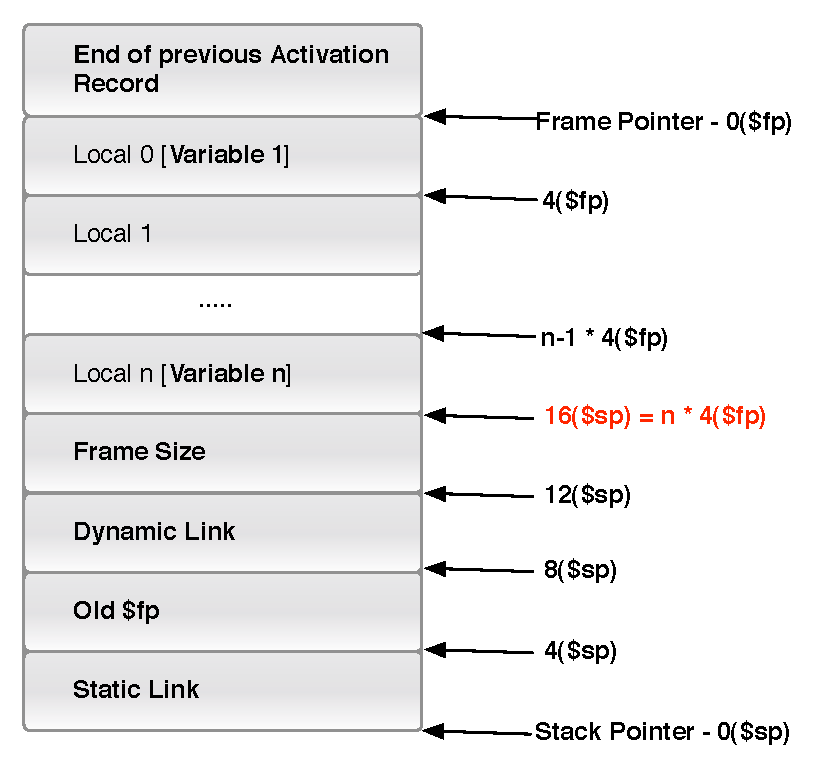
\includegraphics[scale=0.6]{ar-include.pdf}
	\caption{Activation Record - Design}
	\label{fig:AR}
\end{figure}

\begin{figure}[p]
	\begin{verbatim}
		enum sys_register {
		    $zero = 0, 
		    $at = 1,	
		    $v0 = 2, $v1 = 3,
		    $a0 = 4, $a1 = 5, $a2 = 6, $a3 = 7,
		    $t0 = 8, $t1 = 9, $t2 = 10, $t3 = 11, $t4 = 12, $t5 = 13, $t6 = 14,	$t7 = 15,					
		    $s0 = 16, $s1 = 17, $s2 = 18, $s3 = 19, $s4 = 20, $s5 = 21, $s6 = 22, $s7 = 23,
		    $t8 = 24, $t9 = 25,
		    $k0 = 26, $k1 = 27,
		    $gp = 28,
		    $sp = 29,
		    $fp = 30,
		    $ra = 31				
		}sys_register;

		typedef struct register_offset {
		    enum sys_register reg;
		    int offset;
		}register_offset;

		typedef union operand {
		    enum sys_register reg;
		    struct register_offset* reg_offset;
		    int constant;
		    char *label;
		}operand;
		
		typedef struct mips_instruction {
		    char *operation;
		    int operand1_type;
		    int operand2_type;
		    int operand3_type;
		    union operand *operand1;
		    union operand *operand2;
		    union operand *operand3;		
		    char *comment;
		    int indent_count;
		    struct mips_instruction *next;
		}mips_instruction;
	\end{verbatim}
	\caption{MIPS Instruction structure}
	\label{fig:mipsinstr}
\end{figure}